% 03_report.tex -- ECO1465 Week 5 report, Tsu Ning Tsao
% Compiled by 00_master.py from inside 03_output/ (all figures, tables and
% numbers.tex are produced by 02_analysis.py; nothing is typed by hand).
\documentclass[11pt]{article}
\usepackage[margin=0.9in]{geometry}
\usepackage{graphicx,booktabs,amsmath,float,caption,subcaption,xcolor}
\usepackage[hidelinks]{hyperref}
\captionsetup{font=small,labelfont=bf,skip=4pt}
\setlength{\parskip}{4pt}\setlength{\parindent}{0pt}
\newcommand{\SageCoef}{0.76}
\newcommand{\SageR}{0.099}
\newcommand{\SageAUC}{0.72}
\newcommand{\SageN}{1,270}
\newcommand{\SageBal}{0.45}
\newcommand{\SoldCoef}{28.0}
\newcommand{\SoldR}{0.104}
\newcommand{\SnextR}{0.017}
\newcommand{\SjointAge}{0.80}
\newcommand{\SjointN}{804}
\newcommand{\SjointR}{0.120}
\newcommand{\SvalR}{0.0013}
\newcommand{\SratioR}{78}
\newcommand{\CageEdu}{-0.22}
\newcommand{\CageJob}{0.17}
\newcommand{\CageFem}{-0.20}
\newcommand{\CfemEdu}{-0.32}
\newcommand{\Nall}{29,418}
\newcommand{\Nnb}{220}
\newcommand{\Nlinked}{2,567}
\newcommand{\Mexempt}{13.3}
\newcommand{\Eexempt}{1.6}
\newcommand{\SEexempt}{0.9}
\newcommand{\Eold}{1.4}
\newcommand{\SEold}{0.7}
\newcommand{\Pold}{0.04}
\newcommand{\Ewid}{0.0}
\newcommand{\SEwid}{0.5}
\newcommand{\Elk}{2.0}
\newcommand{\Elkage}{2.5}
\newcommand{\Mun}{3.8}
\newcommand{\Eun}{1.5}
\newcommand{\Pun}{0.07}
\newcommand{\Eco}{-3.3}
\newcommand{\Pco}{0.36}
\newcommand{\Mbr}{2.0}
\newcommand{\Ebr}{2.0}
\newcommand{\Pbr}{0.06}
\newcommand{\Nbr}{814}
\newcommand{\Fyoung}{12}
\newcommand{\Fold}{50}


\begin{document}
\begin{center}
{\large\bfseries Do Local Chiefs Grant More Discretionary Tax Exemptions? Evidence from a Randomized Tax Collection Experiment in Kananga, D.R.\ Congo}\\[6pt]
\textbf{Name:} Tsu Ning Tsao \qquad \textbf{Student Number:} 1012713137
\end{center}

\section*{One-Paragraph Research Summary}
\textbf{Research question.} Does replacing central state collectors (Central, \texttt{treatment}\,=\,1) with local city chiefs (Local, \texttt{treatment}\,=\,2) increase or decrease favoritism in property-tax collection, measured as tax exemptions, and for which households is the effect larger? \textbf{Data.} Replication files of Bal\'an et al.\ (2022): the 2018 tax roll (compound level; \Nall{} compounds in \Nnb{} Central or Local neighborhoods), merged with the 2017 household baseline (\Nlinked{} compounds linked), the pre-randomization chief survey and the endline survey. Treatment is randomized at the neighborhood level within geographic strata. \textbf{Outcome and treatment.} $Y$ = \texttt{exempt} (1 if the compound is recorded as exempt), split by stated reason into old age (\emph{Troisi\`eme \^age}) and widowhood (\emph{Veuve}); secondary outcomes are old-age exemptions granted to compounds whose respondent is under 60 and the endline self-reported bribe. $D$ = Local. Because assignment is random, Local minus Central is the causal effect; no IV is needed. Local raises exemptions by \Eexempt{} pp (SE \SEexempt) over a Central mean of \Mexempt\%, almost entirely through old-age exemptions (\Eold{} pp, SE \SEold, $p=\Pold$); widow exemptions do not change (\Ewid{} pp, SE \SEwid).

\section*{1. Two DAGs: the experiment and the biased sample}

\begin{figure}[H]
\centering
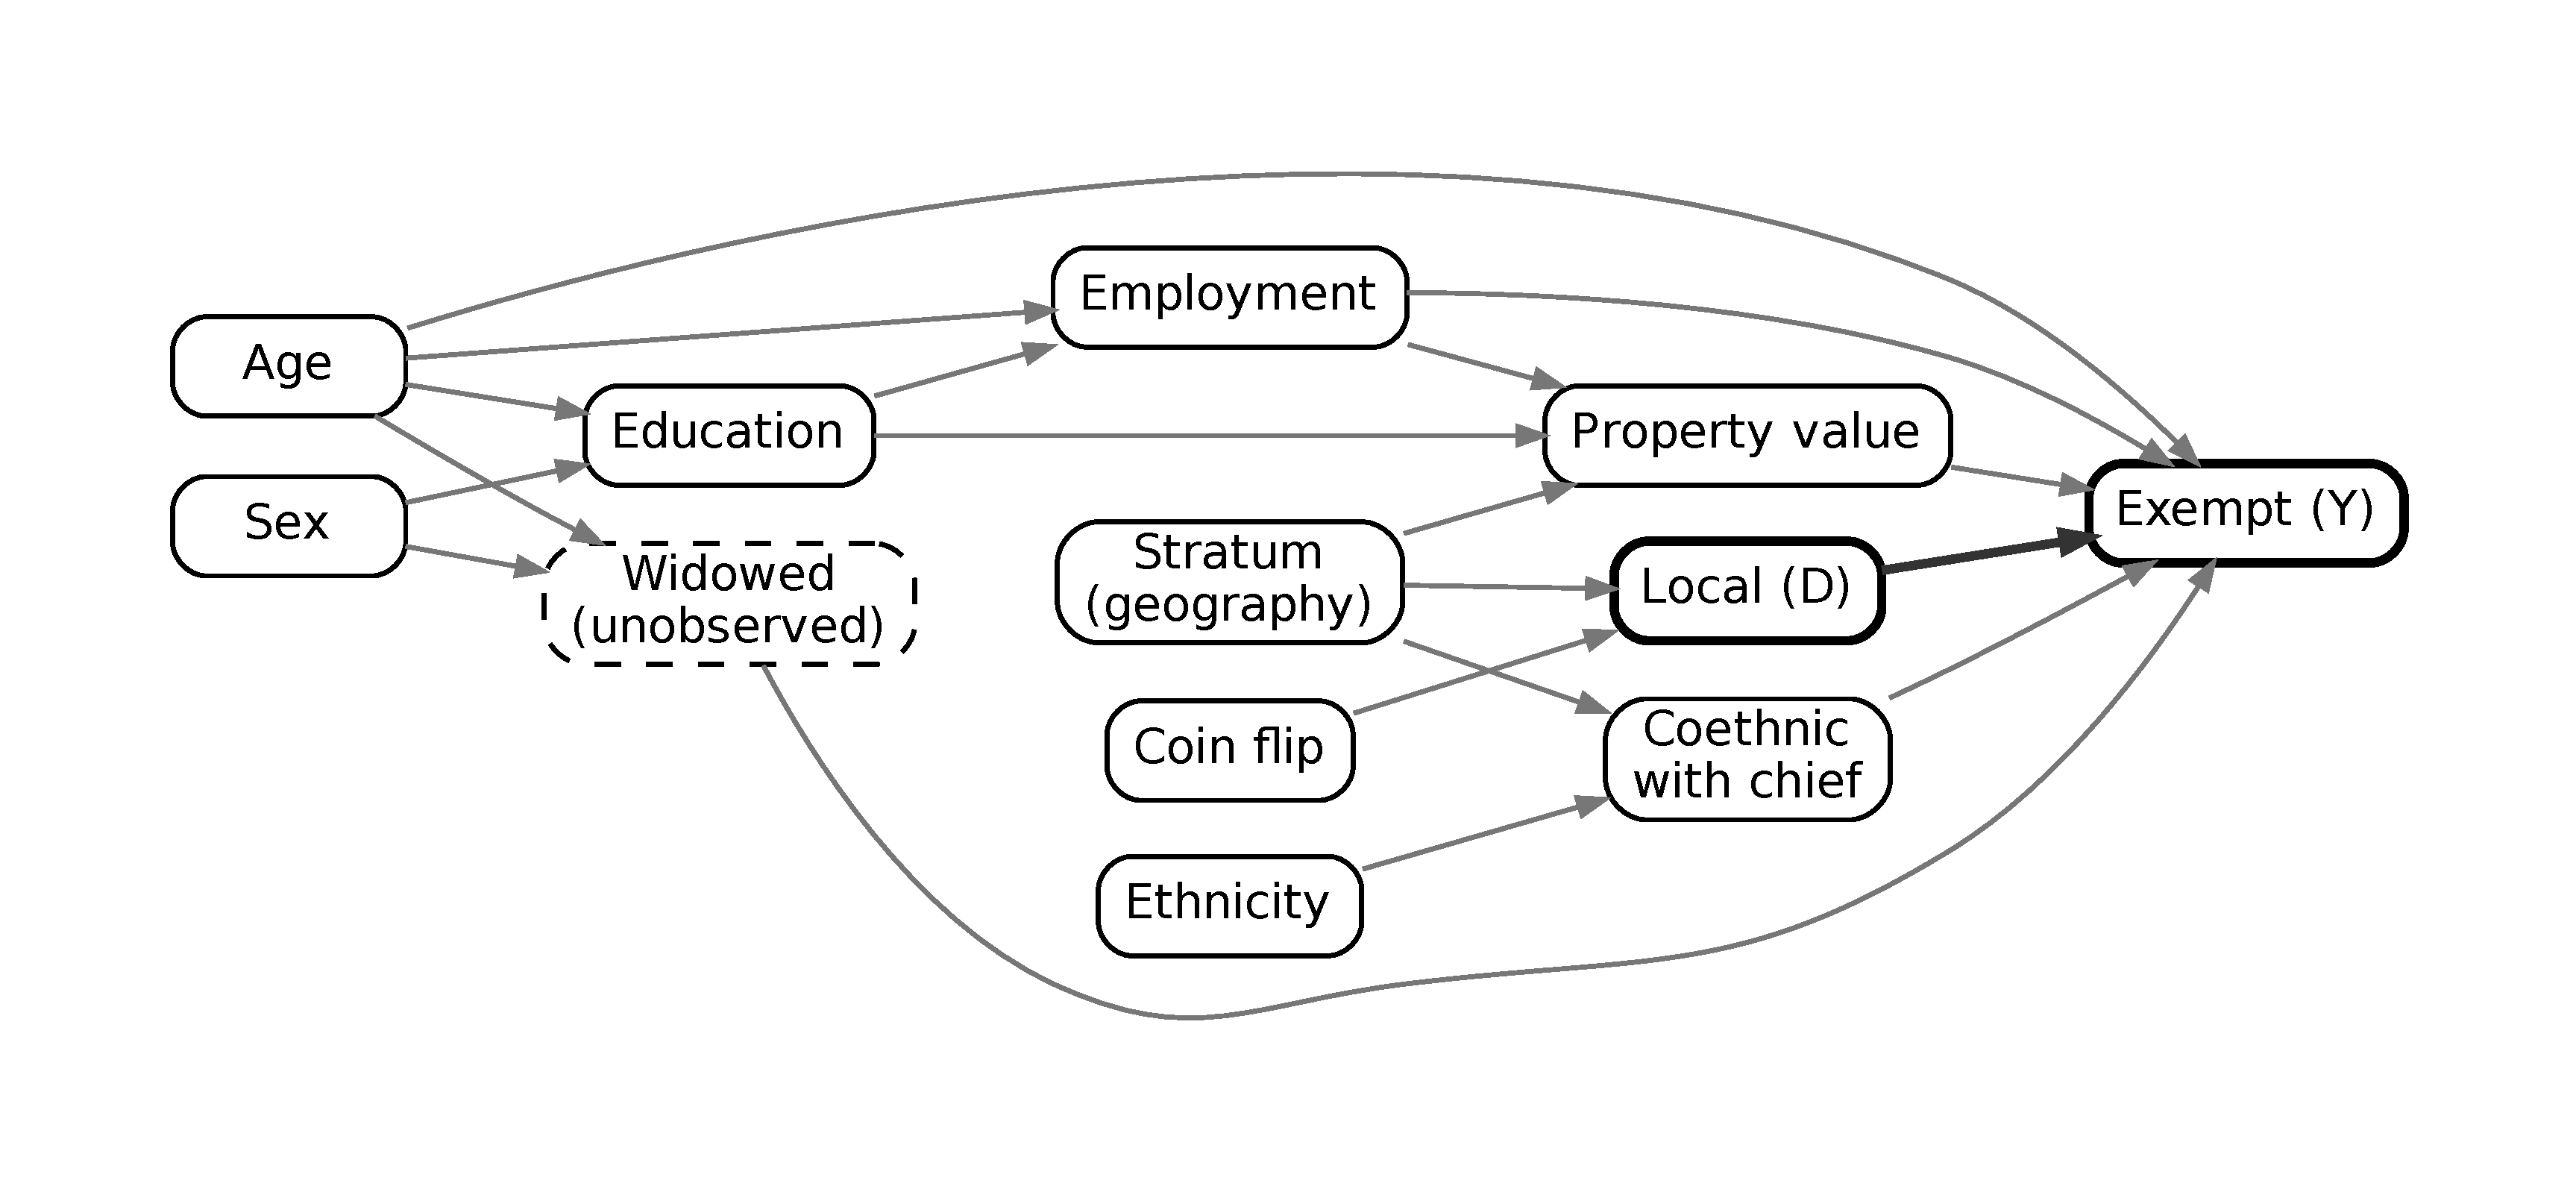
\includegraphics[width=0.86\textwidth]{Figure1a_DAG1_experiment.pdf}
\caption{DAG 1 -- the experiment. $D$ has two parents only: the coin flip and the randomization stratum.}
\end{figure}
\vspace{-6pt}
\textbf{DAG 1.} The baseline covariates are not independent of each other, and the graph draws those links. Age drives widowhood (unobserved in the data), education (older cohorts have less schooling) and employment; sex drives widowhood and education; education and employment drive property value; ethnicity and geography (stratum) together determine whether a household is a coethnic of its chief. In the linked baseline, age correlates $\CageEdu$ with education, $\CageJob$ with having no job and $\CageFem$ with being female (Table~2). These links create many paths among the $X$'s, but none of them enters $D$: the only arrows into $D$ come from the coin flip and from the stratum, and the stratum is held fixed with stratum fixed effects. Every path from $D$ to $Y$ other than $D\to Y$ is therefore closed, so the stratum-adjusted difference in means identifies the ATE. Consistent with this, age is balanced across arms (balance $p=\SageBal$, Table~1), and adding age to the regression barely moves the estimate in the linked sample (\Elk{} pp without, \Elkage{} pp with).

\begin{figure}[H]
\centering
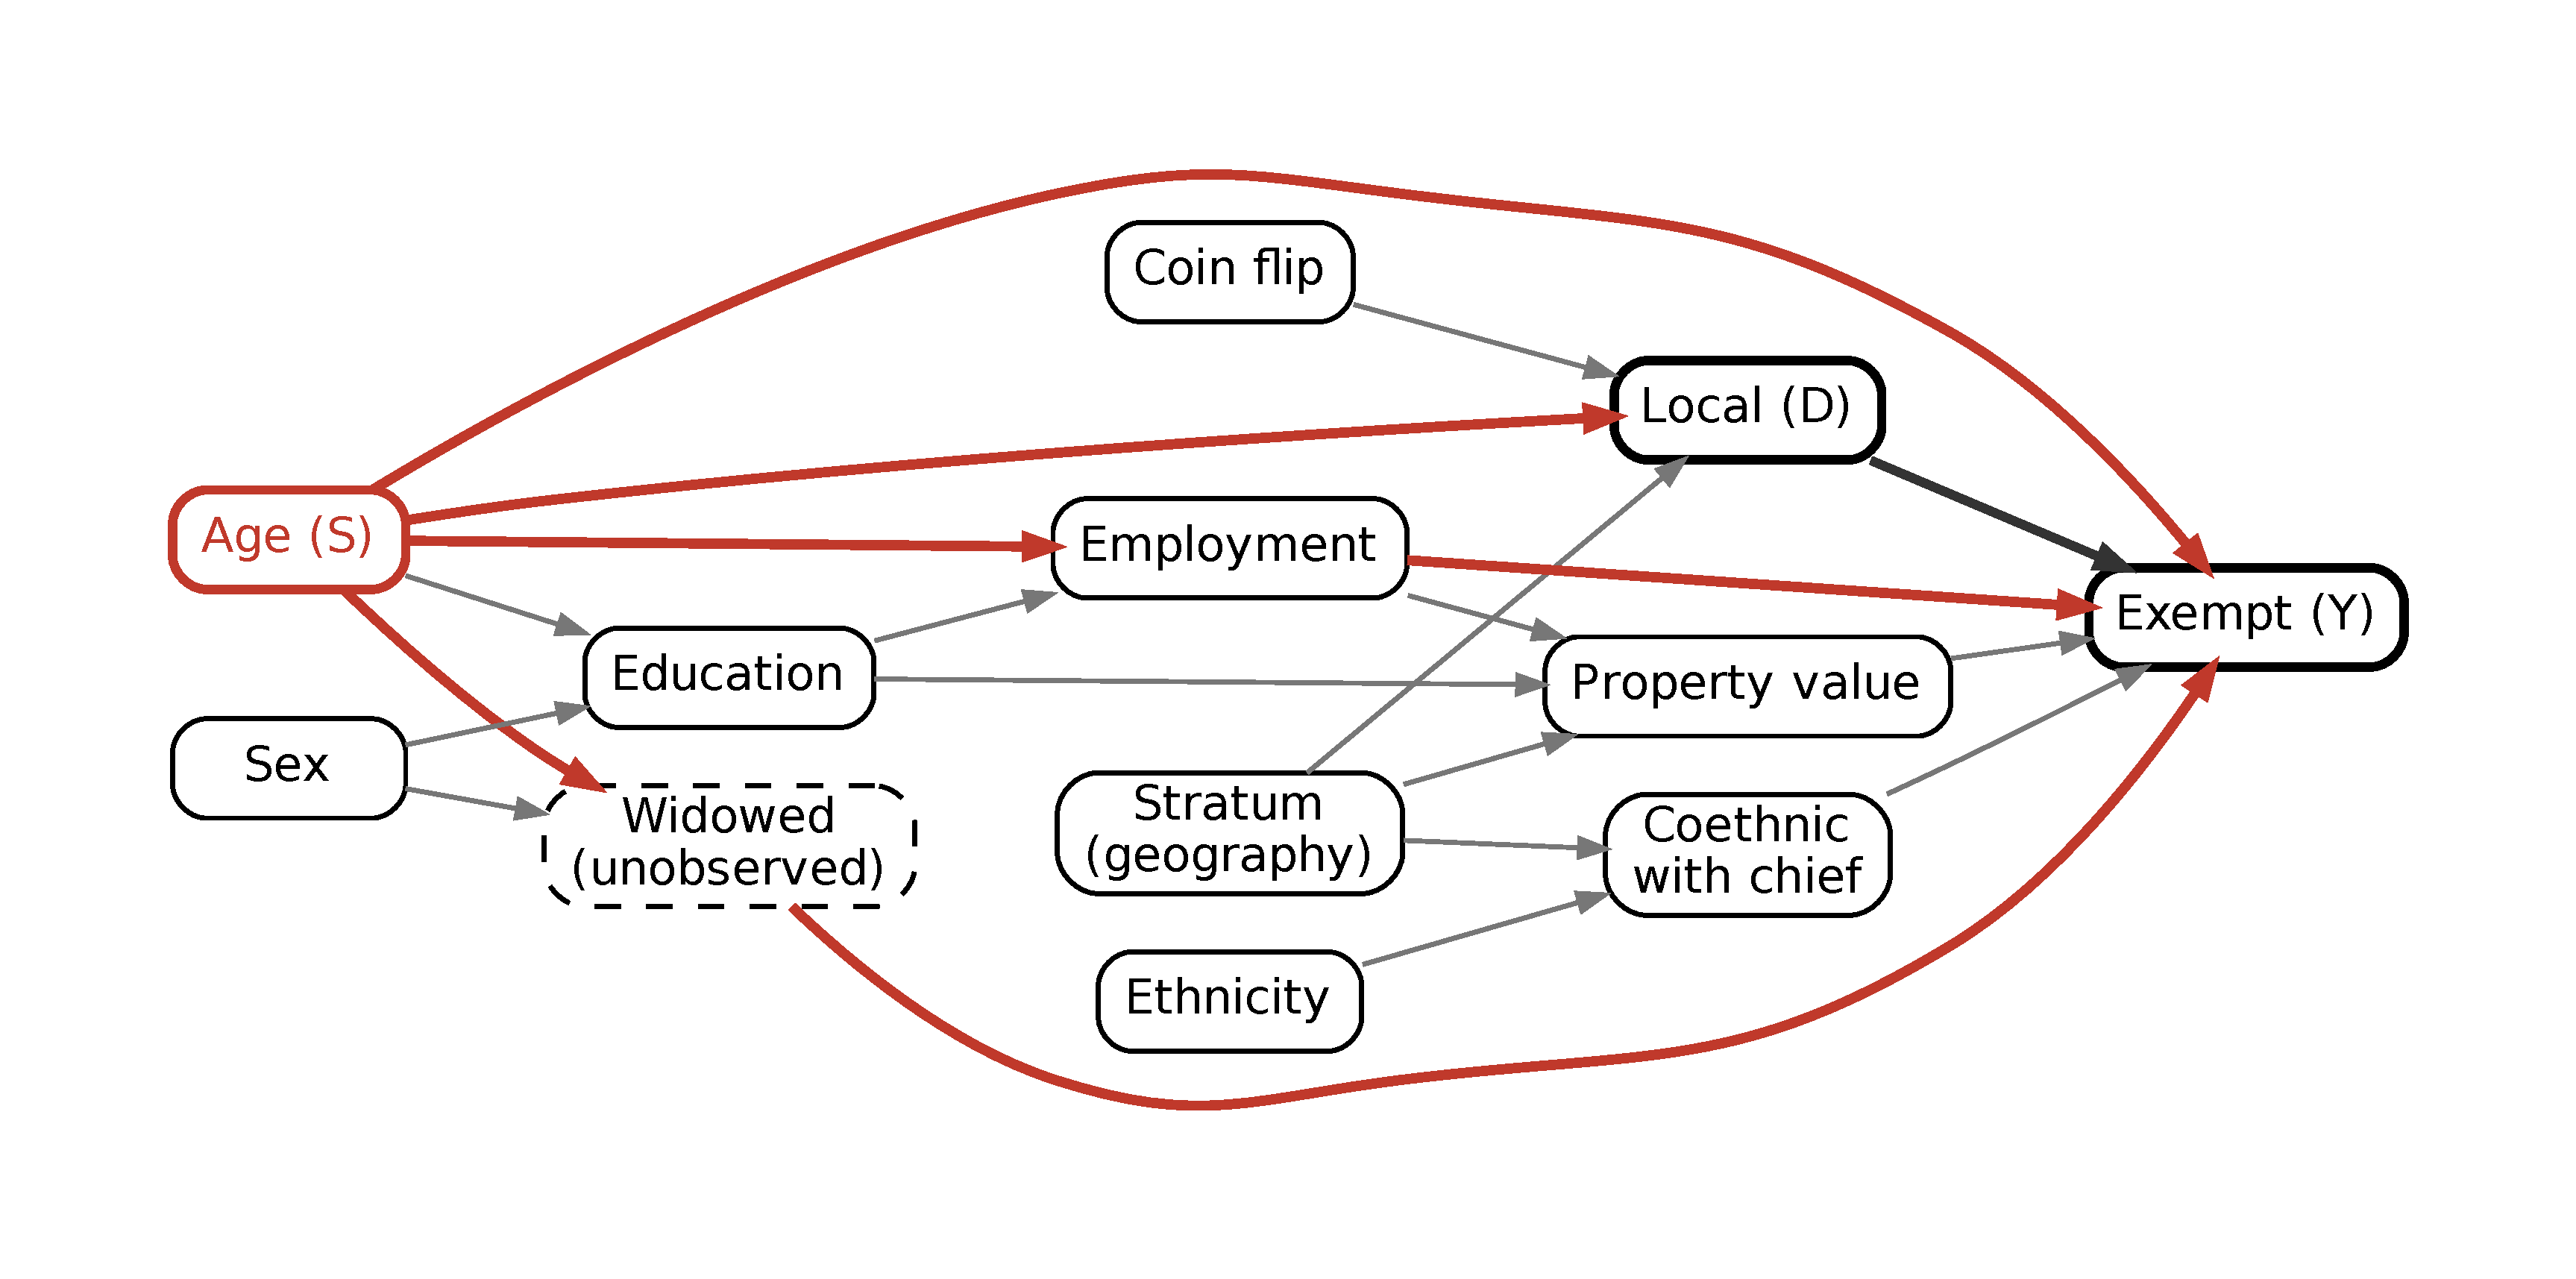
\includegraphics[width=0.86\textwidth]{Figure1b_DAG2_biased.pdf}
\caption{DAG 2 -- the biased sample. Selection on $S$ = age adds $S\to D$; open backdoor paths in red.}
\end{figure}
\vspace{-6pt}
\textbf{DAG 2.} Adding $S\to D$ with $S$ = age opens three backdoor paths, because age reaches $Y$ both directly and through the $X$'s it causes: $D\leftarrow S\to Y$ (legal old-age exemption), $D\leftarrow S\to \text{Widowed}\to Y$ and $D\leftarrow S\to \text{Employment}\to Y$. $S$ is a common cause on all three, so conditioning on $S$ alone (plus the stratum) blocks them all; widowhood and employment need not be controlled for, which matters because widowhood is not observed. Without controlling for $S$, Local neighborhoods would hold more older households, who are exempted more for legitimate reasons, and the difference in means would overstate the effect of chiefs on exemptions. Controlling for employment or education instead of age would not be enough, because $D\leftarrow S\to Y$ would stay open.

\begin{figure}[H]
\centering
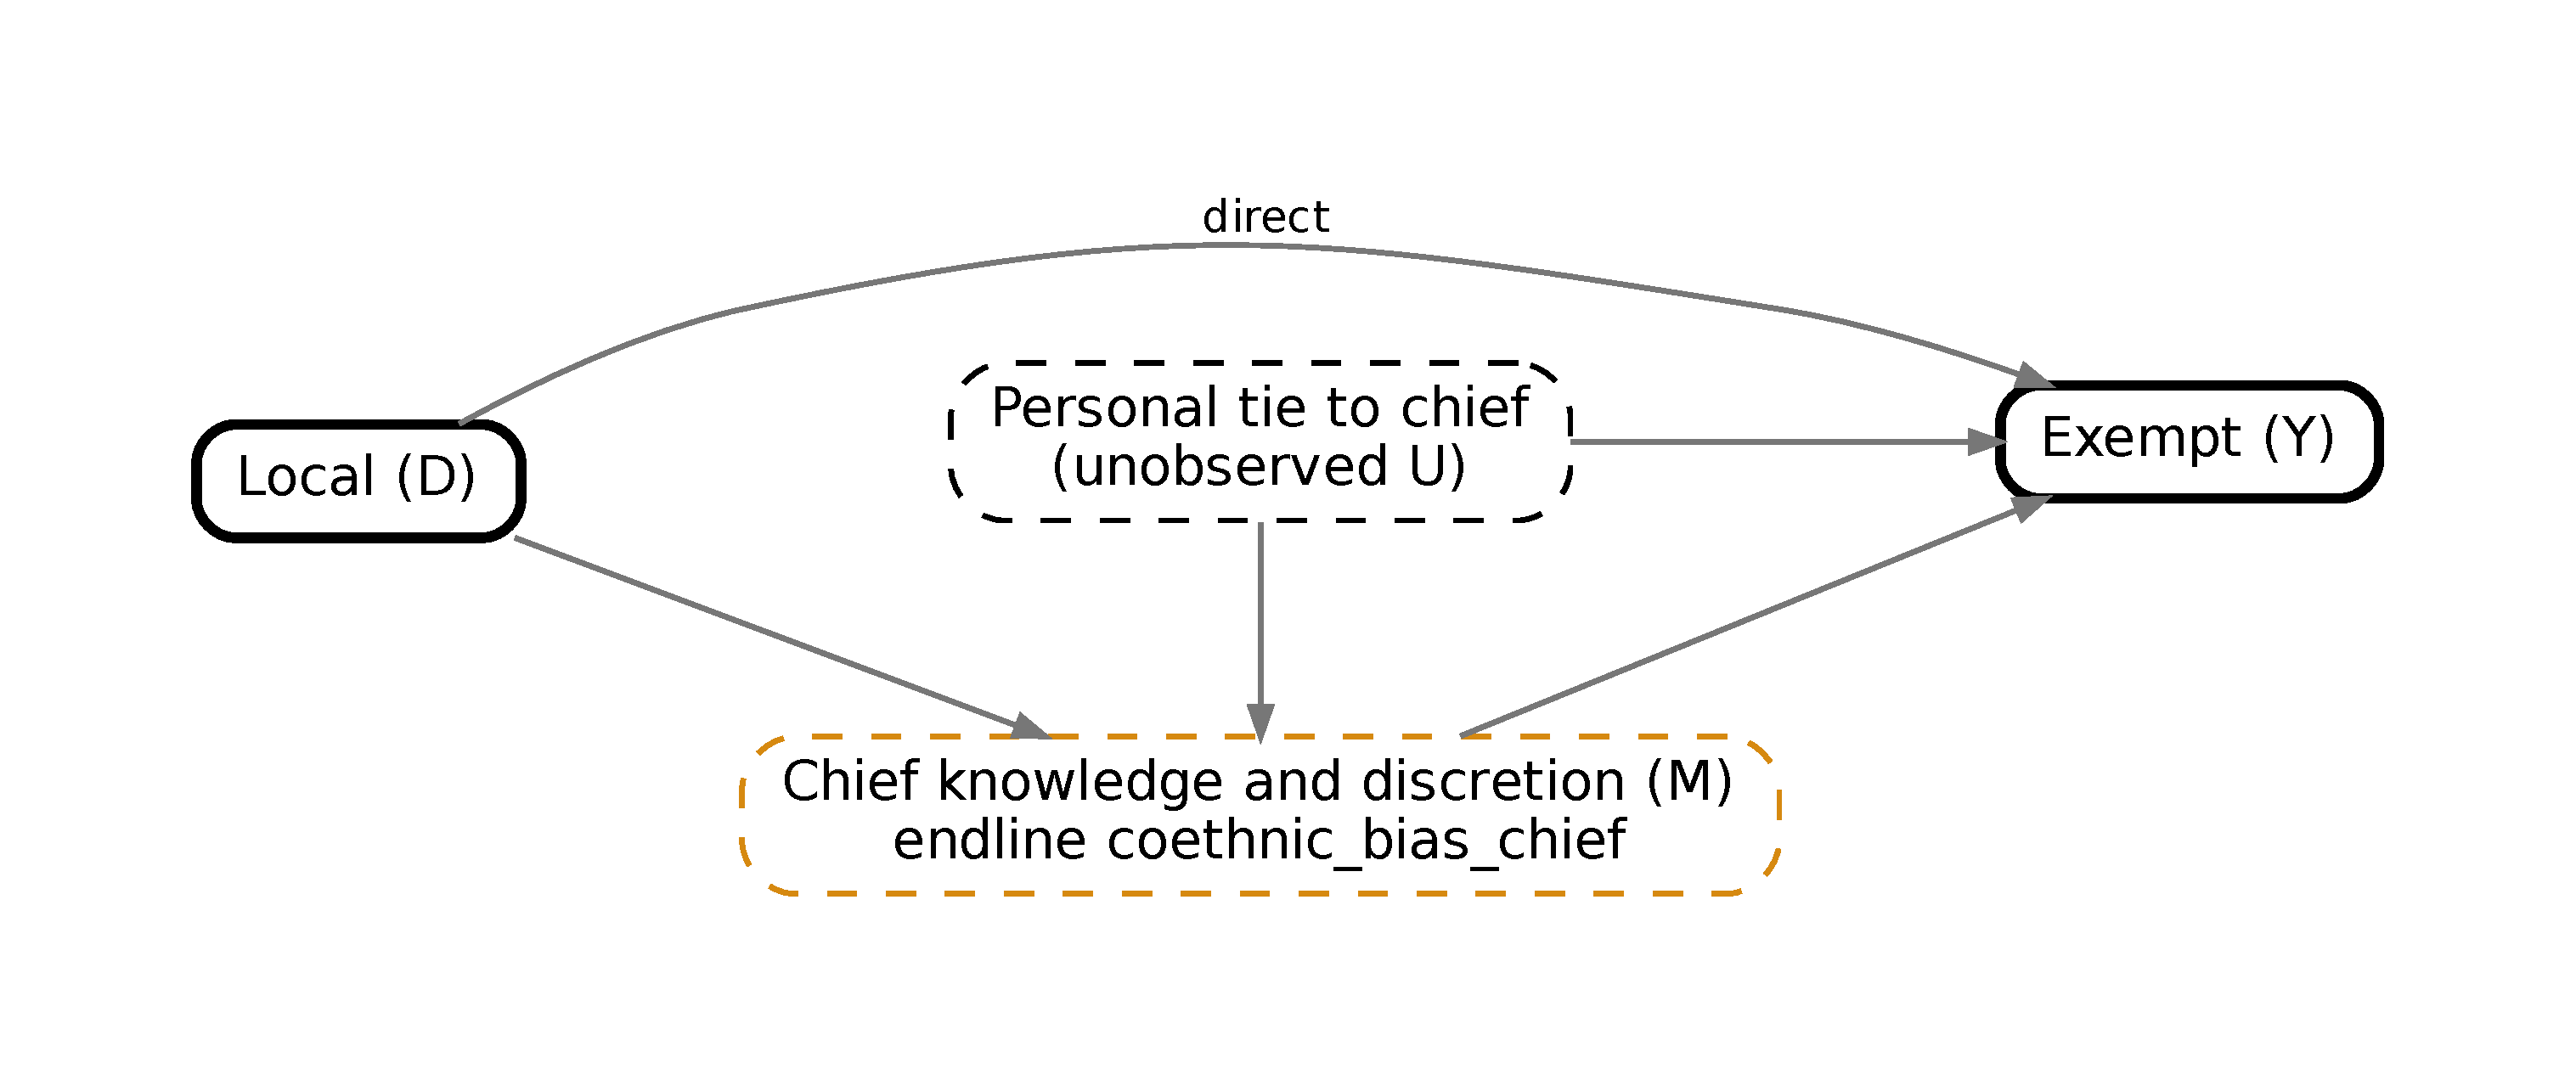
\includegraphics[width=0.78\textwidth]{Figure1c_DAG3_mediator.pdf}
\caption{DAG 3 -- mediator and collider. $M$ is measured after assignment; do not control for it.}
\end{figure}
\vspace{-6pt}
\textbf{DAG 3.} Chiefs plausibly change exemptions through what they know about each household and the discretion they use ($M$), proxied in the endline by \texttt{coethnic\_bias\_chief} (from \texttt{exempt\_tribe}, an outcome in the paper's Table~5). $M$ is measured after assignment and lies on $D\to M\to Y$: controlling for it removes part of the effect. It is also a collider on $D\to M\leftarrow U\to Y$, where $U$ is an unobserved personal tie to the chief, so conditioning on it opens a non-causal path. For heterogeneity I therefore use a pre-treatment coethnic indicator (baseline tribe equals the chief's tribe in the pre-randomization chief survey), not \texttt{coethnic\_bias\_chief}.

\section*{2. Candidate selection variable $S$}
\textbf{$S$ = age of the baseline respondent} (\texttt{age}, household baseline survey, 2017), measured before the 2018 campaign and before assignment. \textbf{Predicts $Y$:} in the Central group, a one-year increase in age raises the exemption probability by \SageCoef{} pp (SE 0.08), $R^2=\SageR$, AUC $=\SageAUC$ ($N=\SageN$); the share exempt rises from \Fyoung\% for respondents under 30 to \Fold\% for those 70 and older (Figure~\ref{fig:age}). Age, used either in years or as a 60-plus indicator ($R^2=\SoldR$), ranks first of eight pre-treatment candidates, with about six times the $R^2$ of the best non-age candidate (no job, $R^2=\SnextR$), and it keeps its size when the other $X$'s are held fixed (joint coefficient \SjointAge{} pp, Table~1), so it is not standing in for employment or education. \textbf{Selection story:} outside the experiment, the government would hand collection to chiefs in older, long-settled neighborhoods where chiefs are entrenched and elderly households are common, so households with high $S$ would be more likely to be treated.

\begin{table}[H]
\centering\footnotesize
\caption{Pre-treatment candidates for $S$, ranked by $R^2$. Coef., SE, $R^2$, AUC: OLS of \texttt{exempt} on the candidate, Central group only, SE clustered by neighborhood. Joint coef.: same regression with all household covariates together ($N=\SjointN$). Balance $p$: Local--Central difference in the candidate with stratum FE.}
\begin{tabular}{lrrrrrrr}
\toprule
Candidate & Coef. & SE & $R^2$ & AUC & Joint coef. & N & Balance $p$ \\
\midrule
Respondent aged 60+ & 0.2803 & 0.0267 & 0.104 & 0.686 &  & 1,270 & 0.154 \\
Age of respondent (years) & 0.0076 & 0.0008 & 0.099 & 0.723 & 0.0080 & 1,270 & 0.451 \\
Respondent has no job & 0.1150 & 0.0280 & 0.017 & 0.575 & 0.0527 & 1,204 & 0.658 \\
Education level & -0.0478 & 0.0148 & 0.009 & 0.442 & 0.0099 & 1,267 & 0.089 \\
Coethnic with chief & 0.0432 & 0.0238 & 0.003 & 0.530 &  & 1,063 & 0.351 \\
Log predicted property value & 0.0129 & 0.0101 & 0.001 & 0.522 & 0.0229 & 1,270 & 0.091 \\
Household size & 0.0010 & 0.0033 & 0.000 & 0.488 & -0.0087 & 1,270 & 0.332 \\
Female respondent & 0.0017 & 0.0297 & 0.000 & 0.501 & 0.0384 & 848 & 0.801 \\
\bottomrule
\end{tabular}

\end{table}

\begin{figure}[H]
\centering
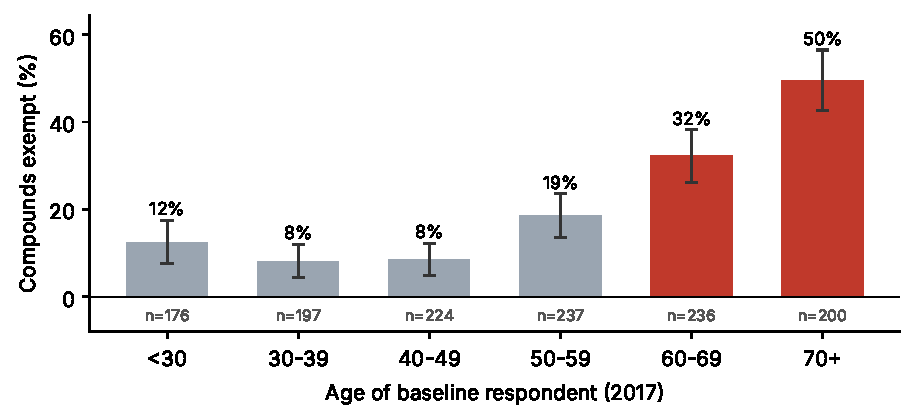
\includegraphics[width=0.66\textwidth]{Figure2_exempt_by_age_central.pdf}
\caption{Share of compounds exempt by age of the baseline respondent, Central neighborhoods only (95\% CI).}\label{fig:age}
\end{figure}

\begin{table}[H]
\centering\footnotesize
\caption{Correlations among pre-treatment covariates (linked baseline sample, both arms).}
\begin{tabular}{lrrrrrrr}
\toprule
 & Age & Female & Education & No job & HH size & Log value & Coethnic \\
\midrule
Age & 1.00 &  &  &  &  &  &  \\
Female & -0.20 & 1.00 &  &  &  &  &  \\
Education & -0.22 & -0.32 & 1.00 &  &  &  &  \\
No job & 0.17 & 0.19 & -0.21 & 1.00 &  &  &  \\
HH size & 0.09 & -0.09 & 0.11 & -0.08 & 1.00 &  &  \\
Log value & -0.01 & 0.08 & 0.14 & 0.03 & 0.04 & 1.00 &  \\
Coethnic & 0.06 & -0.01 & -0.07 & -0.01 & -0.01 & -0.03 & 1.00 \\
\bottomrule
\end{tabular}

\end{table}

\section*{3. Do operation vs.\ statistical conditioning}
$P(Y=1\mid D=\text{Local})$ is the exemption rate among compounds that happen to be in Local neighborhoods: it is an association and includes anything else that differs between the groups. $P(Y=1\mid do(D=\text{Local}))$ is the exemption rate if every neighborhood were set to Local, which deletes all arrows into $D$; it is the causal quantity. In DAG~1 the two are equal, because within a stratum the coin flip is the only parent of $D$, so the Local group is a random draw from the same population. In DAG~2 they differ: conditioning on $D=\text{Local}$ selects older households, so $P(Y\mid D)$ mixes the chief effect with legitimate old-age exemptions. The intervention is recovered by adjusting for $S$:
\[
P\big(Y=1\mid do(D=d)\big)=\sum_{s} P\big(Y=1\mid D=d,\,S=s\big)\,P(S=s).
\]

\end{document}
